%% GENERATED by tools/from_docs.py from stepss-docs. Do not edit by hand:
%% edit the page named below in stepss-docs and regenerate.
%% source: stepss-docs/src/content/docs/developer/cg-studio.mdx

\chapter{CODEGEN Studio}\label{doc:cg-studio}

CODEGEN Studio is a browser-based visual editor for assembling \hyperref[ch-user_models]{User-Defined Models} using the \hyperref[ch-libray_blocks]{CODEGEN block library}. Instead of writing DSL files by hand, you drag blocks onto a canvas, connect them, fill in metadata, and export a valid \texttt{.txt} file ready for the \texttt{codegen} binary.

\section{Installation}\label{cg-studio:installation}

\texttt{pip\ install\ stepss-cg-studio}, then run \texttt{cg-studio}. See
\hyperref[ch-install]{Installing CODEGEN Studio}
for the Python version it needs, the address it serves, and why the \textbf{Run
Codegen} button needs a \texttt{codegen} executable you supply yourself.

\subsection{CLI options}\label{cg-studio:cli-options}

\begin{Verbatim}
cg-studio --port 9000       # use a different port
cg-studio --host 0.0.0.0    # allow network access
cg-studio --no-browser      # start server without opening browser
\end{Verbatim}

\subsection{Install from source (development)}\label{cg-studio:install-from-source-development}

\begin{Verbatim}
git clone https://github.com/SPS-L/stepss-cg-studio
cd stepss-cg-studio
pip install -e ".[dev]"
cg-studio
\end{Verbatim}

\section{Interface Overview}\label{cg-studio:interface-overview}

\begin{figure}[htbp]
\centering
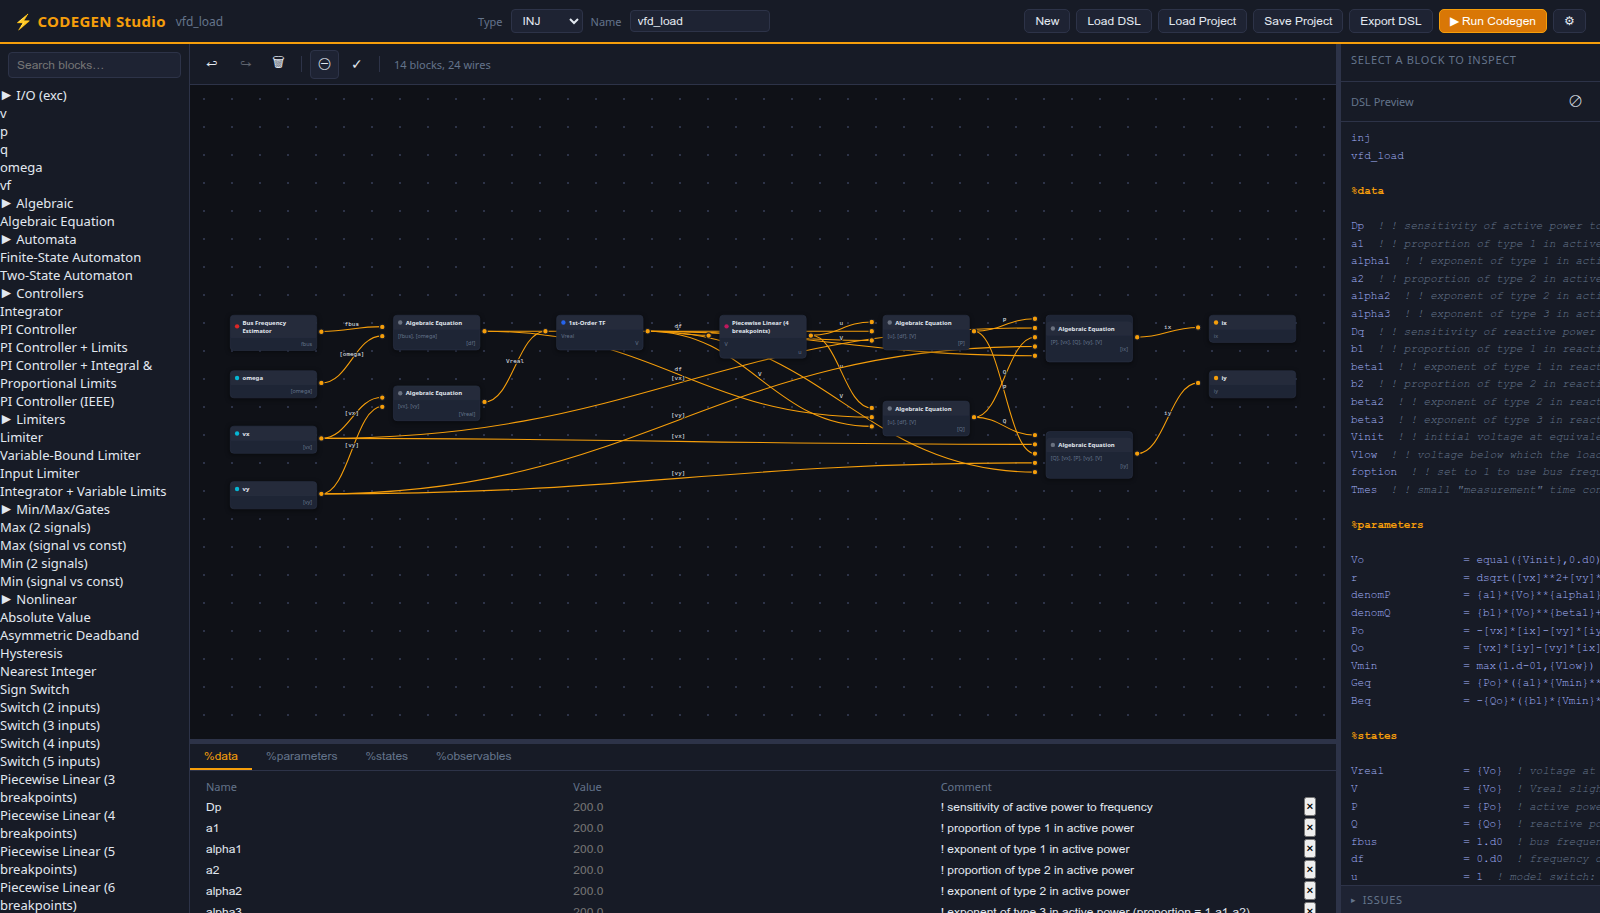
\includegraphics[width=0.98\linewidth]{figures/cg-studio-editor}
\caption{The CODEGEN Studio editor with the vfd\_load injector loaded: the searchable block palette on the left, a canvas of 14 blocks joined by 24 wires in the centre with a first-order transfer function selected, the block inspector and a syntax-highlighted DSL preview on the right, and the \%data metadata table along the bottom.}
\end{figure}

The interface has three columns:

{\def\LTcaptype{none} % do not increment counter
\begin{small}\begin{longtable}[]{@{}
  >{\raggedright\arraybackslash}p{(\linewidth - 6\tabcolsep) * \real{0.2287}}
  >{\raggedright\arraybackslash}p{(\linewidth - 6\tabcolsep) * \real{0.2450}}
  >{\raggedright\arraybackslash}p{(\linewidth - 6\tabcolsep) * \real{0.5263}}
@{}}
\toprule\noalign{}
\begin{minipage}[b]{\linewidth}\raggedright
Area
\end{minipage} & \begin{minipage}[b]{\linewidth}\raggedright
Location
\end{minipage} & \begin{minipage}[b]{\linewidth}\raggedright
Purpose
\end{minipage} \\
\midrule\noalign{}
\endhead
\bottomrule\noalign{}
\endlastfoot
\textbf{Block palette} & Left sidebar & Searchable catalogue of all CODEGEN blocks, grouped by category \\
\textbf{Canvas} & Center & Drag-and-drop block diagram with connection wires \\
\textbf{Metadata tabs} & Below canvas & Editable tables for \texttt{\%data}, \texttt{\%parameters}, \texttt{\%states}, \texttt{\%observables} \\
\textbf{Block inspector} & Right panel (top) & Edit output signal names and block arguments for the selected block \\
\textbf{DSL preview} & Right panel (bottom) & Live syntax-highlighted preview of the generated DSL code \\
\textbf{Topbar} & Top & Model type/name selectors, file operations, and settings \\
\end{longtable}\end{small}
}

\begin{center}\rule{0.5\linewidth}{0.5pt}\end{center}

\section{Creating a Model}\label{cg-studio:creating-a-model}

\subsection{1. Choose the Model Type and Name}\label{cg-studio:choose-the-model-type-and-name}

Use the \textbf{Type} dropdown in the topbar to select the model category:

{\def\LTcaptype{none} % do not increment counter
\begin{small}\begin{longtable}[]{@{}llll@{}}
\toprule\noalign{}
Type & Description & Mandatory outputs & Colour theme \\
\midrule\noalign{}
\endhead
\bottomrule\noalign{}
\endlastfoot
\textbf{EXC} & Excitation controller & \texttt{vf} & Blue \\
\textbf{TOR} & Torque controller & \texttt{tm} & Green \\
\textbf{INJ} & Current injector & \texttt{ix}, \texttt{iy} & Orange \\
\textbf{TWOP} & Two-port device & \texttt{ix1}, \texttt{iy1}, \texttt{ix2}, \texttt{iy2} & Purple \\
\end{longtable}\end{small}
}

\textbf{New} in the topbar asks for the type before it clears the canvas, so a fresh
model starts with the right RAMSES inputs and outputs already seeded.

\begin{figure}[htbp]
\centering
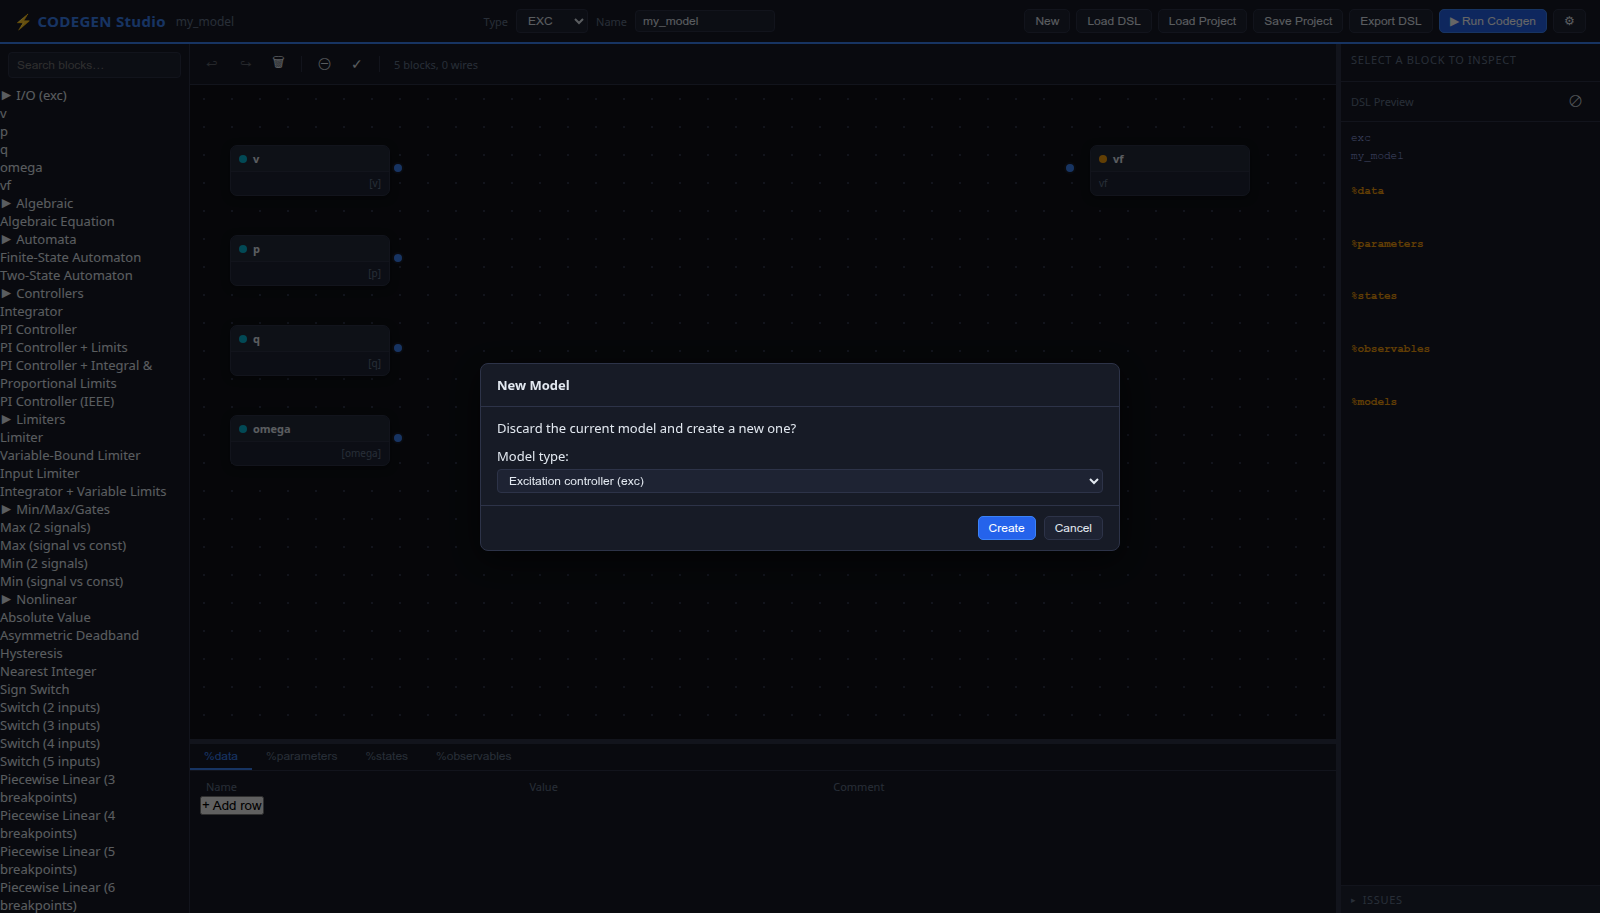
\includegraphics[width=0.98\linewidth]{figures/cg-studio-new-model}
\caption{The New Model dialog over the editor.}
\end{figure}

The UI accent colour changes to reflect the active model type. Type the model name (max 20 characters, the limit CODEGEN itself enforces) in the \textbf{Name} field next to the dropdown.

\begin{docsnote}{Model type determines available inputs}

Each model type exposes a different set of RAMSES input variables in the palette's \textbf{I/O (\texttt{modelType})} category:

{\def\LTcaptype{none} % do not increment counter
\begin{small}\begin{longtable}[]{@{}
  >{\raggedright\arraybackslash}p{(\linewidth - 6\tabcolsep) * \real{0.2068}}
  >{\raggedright\arraybackslash}p{(\linewidth - 6\tabcolsep) * \real{0.4569}}
  >{\raggedright\arraybackslash}p{(\linewidth - 6\tabcolsep) * \real{0.3364}}
@{}}
\toprule\noalign{}
\begin{minipage}[b]{\linewidth}\raggedright
Type
\end{minipage} & \begin{minipage}[b]{\linewidth}\raggedright
Palette inputs
\end{minipage} & \begin{minipage}[b]{\linewidth}\raggedright
Mandatory outputs
\end{minipage} \\
\midrule\noalign{}
\endhead
\bottomrule\noalign{}
\endlastfoot
\texttt{exc} & \texttt{v}, \texttt{p}, \texttt{q}, \texttt{omega} & \texttt{vf} \\
\texttt{tor} & \texttt{p}, \texttt{omega} & \texttt{tm} \\
\texttt{inj} & \texttt{vx}, \texttt{vy}, \texttt{omega} & \texttt{ix}, \texttt{iy} \\
\texttt{twop} & \texttt{vx1}, \texttt{vy1}, \texttt{vx2}, \texttt{vy2}, \texttt{omega1}, \texttt{omega2} & \texttt{ix1}, \texttt{iy1}, \texttt{ix2}, \texttt{iy2} \\
\end{longtable}\end{small}
}

The \texttt{exc} type also reserves \texttt{if} as a RAMSES name (usable in DSL expressions such as \texttt{{[}if{]}}) but it is not a palette input. See \hyperref[ch-user_models]{User-Defined Models} for the complete list of reserved names.

\end{docsnote}

\subsection{2. Add Blocks to the Canvas}\label{cg-studio:add-blocks-to-the-canvas}

The left palette lists all available blocks from the \hyperref[ch-libray_blocks]{CODEGEN Blocks} reference, organised by category (Transfer Functions, Limiters, Controllers, etc.).

\begin{enumerate}
\def\labelenumi{\arabic{enumi}.}
\tightlist
\item
  \textbf{Search} by typing in the search box at the top of the palette
\item
  \textbf{Expand} a category by clicking its header
\item
  \textbf{Drag} a block from the palette onto the canvas
\end{enumerate}

Each block appears as a node with input ports on the left and output ports on the right. A coloured dot indicates the block category.

\subsection{3. Connect Blocks}\label{cg-studio:connect-blocks}

Click and drag from an \textbf{output port} (right side) of one block to an \textbf{input port} (left side) of another. A wire appears showing the signal flow. The connection assigns a signal name that links the two blocks in the generated DSL.

\begin{itemize}
\tightlist
\item
  Each input port accepts exactly one incoming wire
\item
  Each output port can fan out to multiple inputs
\item
  The status bar below the canvas toolbar shows the current block and wire count
\end{itemize}

\begin{docsnote}{Cycle detection}

If your connections form a cycle, the status bar shows \textbf{``Cycle detected''} in red
in place of the block and wire count. Feedback loops in control systems are valid
in RAMSES, but the loop must be broken by declaring the fed-back signal as a
\texttt{\%state} with an explicit initial value. See
\hyperref[ch-user_models]{User-Defined Models, States} for details.

The warning is advisory: it does not stop you exporting or running the model. It
also does not yet account for a loop that a \texttt{\%state} already breaks, so a valid
model with feedback can show it. Two of the editor's own example models do,
\texttt{exc\_AC1A} among them. Read it as a prompt to check your states rather than as a
verdict.

\end{docsnote}

\subsection{4. Edit Block Properties}\label{cg-studio:edit-block-properties}

Click a block on the canvas to select it. The \textbf{Block Inspector} (right panel) shows:

\begin{itemize}
\tightlist
\item
  \textbf{Output signal names}: one editable field per output port. The default auto-generated name (e.g., \texttt{tf11}, \texttt{int2}) can be renamed to any valid identifier. This is the state name that appears in the DSL.
\item
  \textbf{Arguments}: block-specific parameters such as gain \texttt{K}, time constant \texttt{T}, or limiter bounds. Values can be:

  \begin{itemize}
  \tightlist
  \item
    A numeric literal: \texttt{1.0}
  \item
    A data reference: \texttt{\{KA\}} (refers to an entry in \texttt{\%data})
  \item
    A Fortran expression: \texttt{\{1/\{omegac\}\}}
  \end{itemize}
\end{itemize}

The \texttt{algeq} (algebraic equation) block has a special \textbf{Expression} field for the equation set to zero.

\begin{figure}[htbp]
\centering
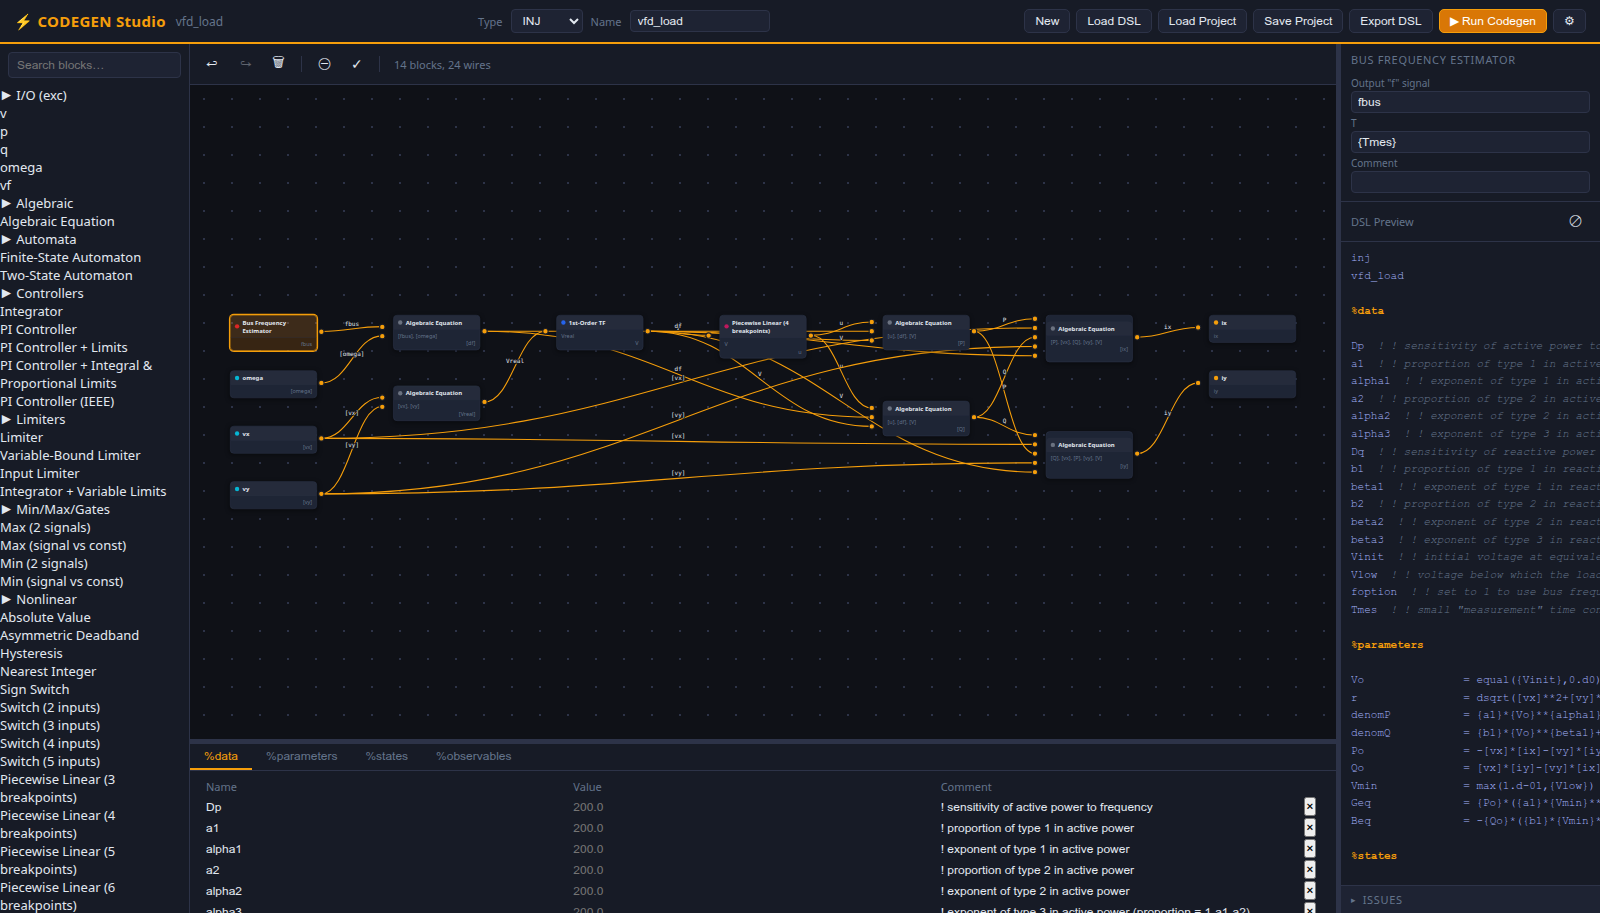
\includegraphics[width=0.98\linewidth]{figures/cg-studio-inspector}
\caption{The CODEGEN Studio editor with a bus frequency estimator block selected on the canvas.}
\end{figure}

\subsection{5. Fill in the Metadata Tables}\label{cg-studio:fill-in-the-metadata-tables}

The four tabs below the canvas correspond to the four metadata sections of a CODEGEN DSL file:

\begin{figure}[htbp]
\centering
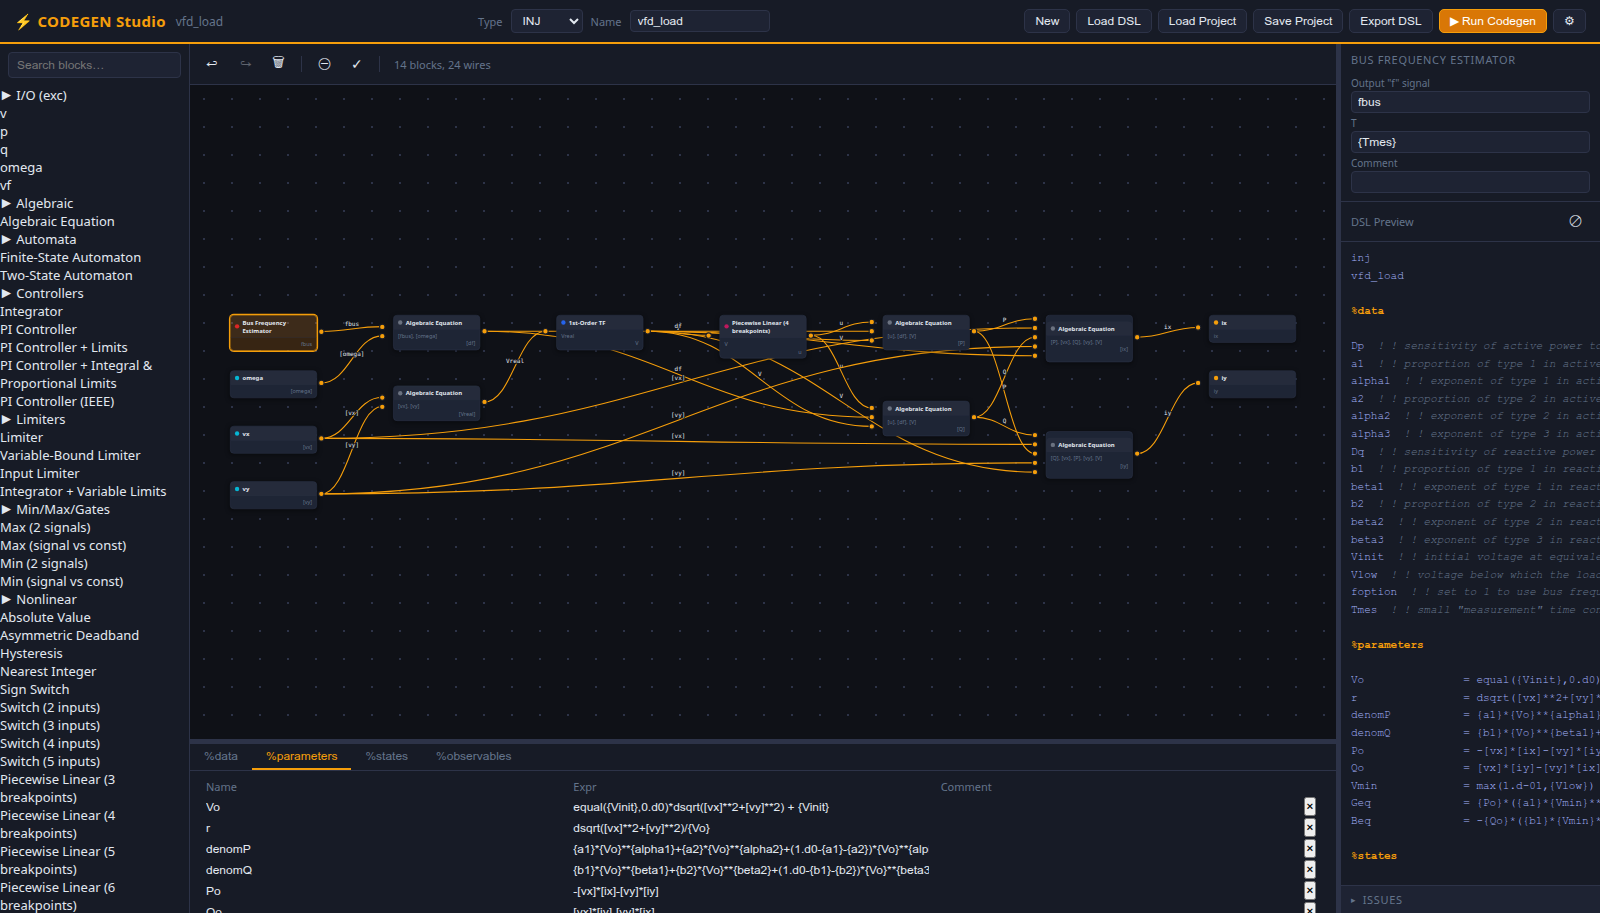
\includegraphics[width=0.98\linewidth]{figures/cg-studio-parameters}
\caption{The \%parameters tab of the metadata panel below the canvas, on the vfd\_load injector.}
\end{figure}

\textbf{\%data}

\textbf{Purpose:} Declare named constants whose values are read from the RAMSES data record at runtime.

{\def\LTcaptype{none} % do not increment counter
\begin{small}\begin{longtable}[]{@{}lll@{}}
\toprule\noalign{}
Column & Description & Example \\
\midrule\noalign{}
\endhead
\bottomrule\noalign{}
\endlastfoot
Name & Identifier (max 20 chars) & \texttt{KA} \\
Value & Optional default & \texttt{200.0} \\
Comment & Annotation & \texttt{AVR\ gain} \\
\end{longtable}\end{small}
}

In block arguments and expressions, reference data values with braces: \texttt{\{KA\}}.

\textbf{\%parameters}

\textbf{Purpose:} Define derived quantities computed once at initialisation from data and initial state values.

{\def\LTcaptype{none} % do not increment counter
\begin{small}\begin{longtable}[]{@{}lll@{}}
\toprule\noalign{}
Column & Description & Example \\
\midrule\noalign{}
\endhead
\bottomrule\noalign{}
\endlastfoot
Name & Identifier & \texttt{Vo} \\
Expr & Fortran expression & \texttt{{[}vf{]}/\{KE\}+{[}vf{]}/\{KA\}} \\
Comment & Annotation & \texttt{initial\ voltage} \\
\end{longtable}\end{small}
}

Use \texttt{{[}name{]}} to reference state/input variables and \texttt{\{name\}} to reference data constants. Multi-line expressions are supported with the \texttt{\&} continuation marker.

\textbf{\%states}

\textbf{Purpose:} Declare the internal state variables of the model and their initial-condition expressions.

{\def\LTcaptype{none} % do not increment counter
\begin{small}\begin{longtable}[]{@{}lll@{}}
\toprule\noalign{}
Column & Description & Example \\
\midrule\noalign{}
\endhead
\bottomrule\noalign{}
\endlastfoot
Name & State identifier & \texttt{avr1} \\
Init & Initial value expression & \texttt{vf/\{KE\}} \\
Comment & Annotation & \texttt{AVR\ integrator} \\
\end{longtable}\end{small}
}

Every block output signal that represents a dynamic state should have a corresponding entry here. The mandatory output states for the selected model type (e.g., \texttt{vf} for EXC) must appear either as block outputs or in \texttt{\%states}.

\textbf{\%observables}

\textbf{Purpose:} List variables to be recorded during simulation. These are typically the states you want to monitor.

{\def\LTcaptype{none} % do not increment counter
\begin{small}\begin{longtable}[]{@{}lll@{}}
\toprule\noalign{}
Column & Description & Example \\
\midrule\noalign{}
\endhead
\bottomrule\noalign{}
\endlastfoot
Name & Observable name & \texttt{vf} \\
\end{longtable}\end{small}
}

Observables do not need expressions. They refer to state names already defined elsewhere in the model.

Click \textbf{``+ Add row''} to append a row. Click the \textbf{x} button on a row to remove it. All edits update the DSL preview in real time.

\subsection{6. Review the DSL Preview}\label{cg-studio:review-the-dsl-preview}

The bottom-right panel shows a \textbf{live syntax-highlighted preview} of the generated DSL code. It updates automatically (with a 600 ms debounce) after every change. The preview uses colour coding:

{\def\LTcaptype{none} % do not increment counter
\begin{small}\begin{longtable}[]{@{}ll@{}}
\toprule\noalign{}
Colour & Meaning \\
\midrule\noalign{}
\endhead
\bottomrule\noalign{}
\endlastfoot
Orange, bold & Section headers (\texttt{\%data}, \texttt{\%parameters}, etc.) \\
Gray, italic & Comments (\texttt{!\ ...}) \\
Blue & Numeric literals \\
Purple & Data/parameter references (\texttt{\{KA\}}) \\
Cyan & State/input references (\texttt{{[}omega{]}}) \\
\end{longtable}\end{small}
}

Click the \textbf{copy button} in the preview header to copy the DSL text to your clipboard.

\begin{center}\rule{0.5\linewidth}{0.5pt}\end{center}

\section{Saving a Project}\label{cg-studio:saving-a-project}

Click \textbf{``Save Project''} in the topbar (or press \textbf{Ctrl+S} / \textbf{Cmd+S}).

The browser downloads a \texttt{.json} file named after your model (e.g., \texttt{simple\_avr.json}) containing the complete project state:

\begin{itemize}
\tightlist
\item
  Model type and name
\item
  All blocks with their positions, arguments, and output signal names
\item
  All wire connections
\item
  All metadata (data, parameters, states, observables)
\end{itemize}

This is a \textbf{lossless format}, every aspect of your canvas layout and configuration is preserved. Use this format for work-in-progress models that you intend to continue editing.

\begin{center}\rule{0.5\linewidth}{0.5pt}\end{center}

\section{Loading a Project}\label{cg-studio:loading-a-project}

Click \textbf{``Load Project''} in the topbar and select a previously saved \texttt{.json} file.

The editor restores the full project state:
- Canvas blocks appear at their saved positions
- All wires are reconnected
- Metadata tables repopulate
- The model type and name update in the topbar
- The colour theme switches to match the model type

A toast notification confirms the load with the model name.

\begin{docsnote}{New vs. Load}

Clicking \textbf{``New''} resets the editor to a blank state. A confirmation dialog (``Discard current model?'') prevents accidental loss of work. If you want to keep your current model, save it first.

\end{docsnote}

\begin{center}\rule{0.5\linewidth}{0.5pt}\end{center}

\section{Importing a DSL File}\label{cg-studio:importing-a-dsl-file}

Click \textbf{``Load DSL''} and select a \texttt{.txt} file written in the \hyperref[ch-user_models]{CODEGEN DSL format}.

The backend parser extracts all sections and blocks from the file, and the editor reconstructs the canvas:

\begin{enumerate}
\def\labelenumi{\arabic{enumi}.}
\tightlist
\item
  Each \texttt{\&\ blockname} in \texttt{\%models} becomes a node on the canvas
\item
  Signal references are resolved into wire connections
\item
  Metadata sections populate the corresponding tabs
\item
  A \textbf{Sugiyama auto-layout} algorithm assigns node positions automatically:

  \begin{itemize}
  \tightlist
  \item
    Blocks are arranged left-to-right by dependency order
  \item
    A three-pass crossing-reduction minimises wire overlaps
  \item
    Feedback loops are detected and handled gracefully
  \end{itemize}
\end{enumerate}

This lets you visually inspect and edit any existing CODEGEN model, including the \hyperref[doc:codegen-examples]{example models}.

\begin{center}\rule{0.5\linewidth}{0.5pt}\end{center}

\section{Checking the Model}\label{cg-studio:checking-the-model}

The \textbf{yes} button on the canvas toolbar runs every structural check at
once, without waiting for an export. Its findings go to the \textbf{Issues} panel in
the right sidebar, which stays there rather than appearing as a dialog, so the
list can be worked through while the canvas is edited. A model with nothing
wrong reports that too, which is the useful half: it is the confirmation that
the two export gates below will not stop you.

\begin{figure}[htbp]
\centering
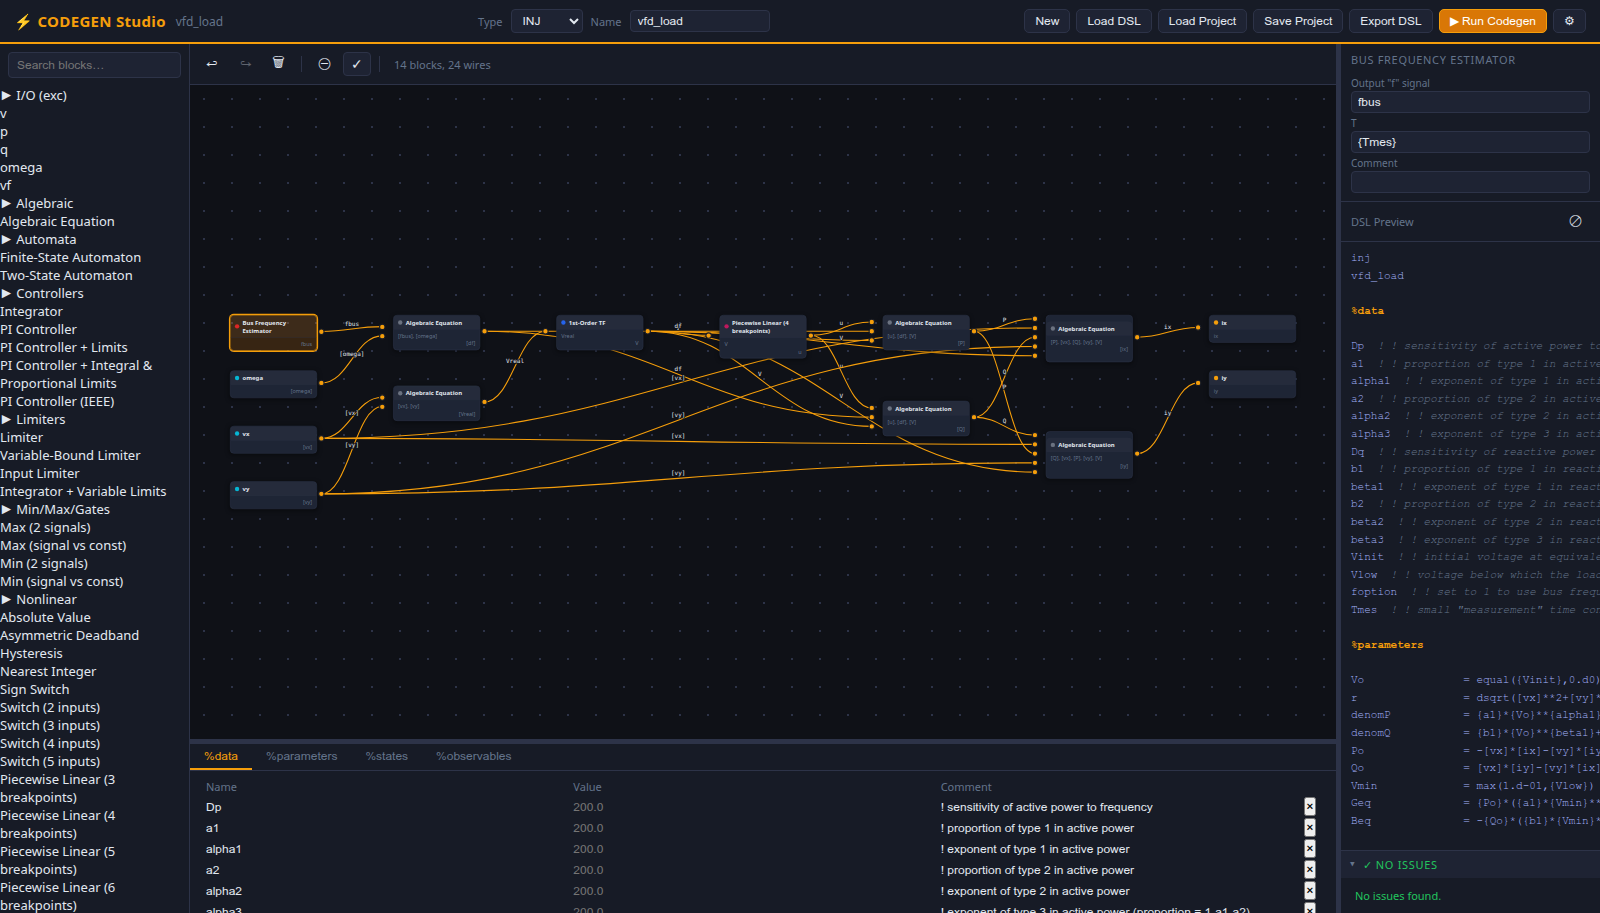
\includegraphics[width=0.98\linewidth]{figures/cg-studio-check}
\caption{The CODEGEN Studio editor after pressing the check button on the canvas toolbar.}
\end{figure}

\begin{center}\rule{0.5\linewidth}{0.5pt}\end{center}

\section{Exporting a DSL File}\label{cg-studio:exporting-a-dsl-file}

Click \textbf{``Export DSL''} to download the generated \texttt{.txt} file.

Export runs two checks, in order. Each raises a dialog you can override with
\textbf{``Export Anyway''} or abandon with \textbf{``Cancel''}.

\textbf{Mandatory outputs.} That every mandatory output state for the selected model
type is produced by at least one block on the canvas:

\begin{quote}
\textbf{Missing Mandatory Outputs}

Missing mandatory outputs for \textbf{exc}: \texttt{vf}

The codegen binary will reject this model.
\end{quote}

\textbf{Floating state connectors.} That no state is referenced by several blocks
without a wire joining them. A state literal sitting on one block's port while the
same name appears elsewhere in the project usually means a connection was left
undrawn on the canvas:

\begin{quote}
\textbf{Floating State Connectors}

The following states are referenced by multiple blocks but the connections are
not wired on the canvas:

\begin{itemize}
\tightlist
\item
  \texttt{Vc} referenced by 2 blocks without a shared wire
\end{itemize}

The emitted DSL may not compile. Wire the connectors up before exporting.
\end{quote}

Note that \textbf{Run Codegen} applies only the first of the two. A model that exports
with a floating-state warning will be sent to the codegen binary without one.

The exported file follows the \hyperref[ch-user_models]{strict DSL section order}: model type, model name, \texttt{\%data}, \texttt{\%parameters}, \texttt{\%states}, \texttt{\%observables}, \texttt{\%models}. Blocks are emitted in topologically-sorted order (dependencies before dependents).

\begin{docsnote}{Round-trip fidelity}

You can import an exported DSL file back into the editor. Unknown block types (not
in the catalogue) are preserved through \texttt{rawArgLines} and re-emitted verbatim, so
the structure survives a round trip even for custom or future blocks.

One exception, in \textbf{comments}: the parser keeps the leading \texttt{!} as part of the
comment text and the emitter adds another, so \texttt{!\ gain} comes back as \texttt{!\ !\ gain},
and a further marker accrues on each pass. It is cosmetic, and \texttt{codegen} ignores
comments, but strip the extra markers before keeping a re-exported file as the
master copy.

\end{docsnote}

\begin{center}\rule{0.5\linewidth}{0.5pt}\end{center}

\section{Running CODEGEN}\label{cg-studio:running-codegen}

Click \textbf{``Run Codegen''} (the accent-coloured button with the play icon) to compile the model into Fortran.

The same mandatory-output validation runs first. If validation passes:

\begin{enumerate}
\def\labelenumi{\arabic{enumi}.}
\tightlist
\item
  The editor generates the DSL text
\item
  The backend writes it to a temporary file and invokes the \texttt{codegen} binary
\item
  On \textbf{success}, a modal displays the generated \texttt{.f90} source code with options to \textbf{``Download .f90''} or \textbf{``Close''}
\item
  On \textbf{failure}, a modal shows the error output from the \texttt{codegen} binary
\end{enumerate}

The downloaded \texttt{.f90} file follows the naming convention \texttt{exc\_simple\_avr.f90} (type prefix + model name) and is ready to compile and link with RAMSES.

\begin{docsnote}{Codegen binary required}

The \texttt{codegen} executable must be installed and its path configured. Click the \textbf{gear icon} in the topbar to open Settings, then set the \textbf{``Codegen binary path''} to the full path of your \texttt{codegen} executable (or just \texttt{codegen} if it is on your system \texttt{PATH}).

\end{docsnote}

\begin{center}\rule{0.5\linewidth}{0.5pt}\end{center}

\section{File Formats Summary}\label{cg-studio:file-formats-summary}

{\def\LTcaptype{none} % do not increment counter
\begin{small}\begin{longtable}[]{@{}
  >{\raggedright\arraybackslash}p{(\linewidth - 8\tabcolsep) * \real{0.1671}}
  >{\raggedright\arraybackslash}p{(\linewidth - 8\tabcolsep) * \real{0.1634}}
  >{\raggedright\arraybackslash}p{(\linewidth - 8\tabcolsep) * \real{0.2894}}
  >{\raggedright\arraybackslash}p{(\linewidth - 8\tabcolsep) * \real{0.3801}}
@{}}
\toprule\noalign{}
\begin{minipage}[b]{\linewidth}\raggedright
Format
\end{minipage} & \begin{minipage}[b]{\linewidth}\raggedright
Extension
\end{minipage} & \begin{minipage}[b]{\linewidth}\raggedright
Use case
\end{minipage} & \begin{minipage}[b]{\linewidth}\raggedright
Lossless?
\end{minipage} \\
\midrule\noalign{}
\endhead
\bottomrule\noalign{}
\endlastfoot
\textbf{Project} & \texttt{.json} & Save/resume editing & Yes, includes canvas positions, all metadata \\
\textbf{DSL} & \texttt{.txt} & Input to \texttt{codegen} binary & Structure only, no canvas layout \\
\textbf{Fortran} & \texttt{.f90} & Output from \texttt{codegen} & Export only, cannot be re-imported \\
\end{longtable}\end{small}
}

\begin{center}\rule{0.5\linewidth}{0.5pt}\end{center}

\section{Keyboard Shortcuts}\label{cg-studio:keyboard-shortcuts}

{\def\LTcaptype{none} % do not increment counter
\begin{small}\begin{longtable}[]{@{}ll@{}}
\toprule\noalign{}
Shortcut & Action \\
\midrule\noalign{}
\endhead
\bottomrule\noalign{}
\endlastfoot
\texttt{Ctrl+S} / \texttt{Cmd+S} & Save project \\
\texttt{Ctrl+Z} / \texttt{Cmd+Z} & Undo \\
\texttt{Ctrl+Y} / \texttt{Cmd+Shift+Z} & Redo \\
\texttt{Delete} / \texttt{Backspace} & Delete selected block \\
\texttt{Escape} & Close any open modal \\
\end{longtable}\end{small}
}

Shortcuts are disabled while typing in text fields.

\begin{center}\rule{0.5\linewidth}{0.5pt}\end{center}

\section{Settings}\label{cg-studio:settings}

Click the \textbf{gear icon} in the topbar to configure:

\begin{figure}[htbp]
\centering
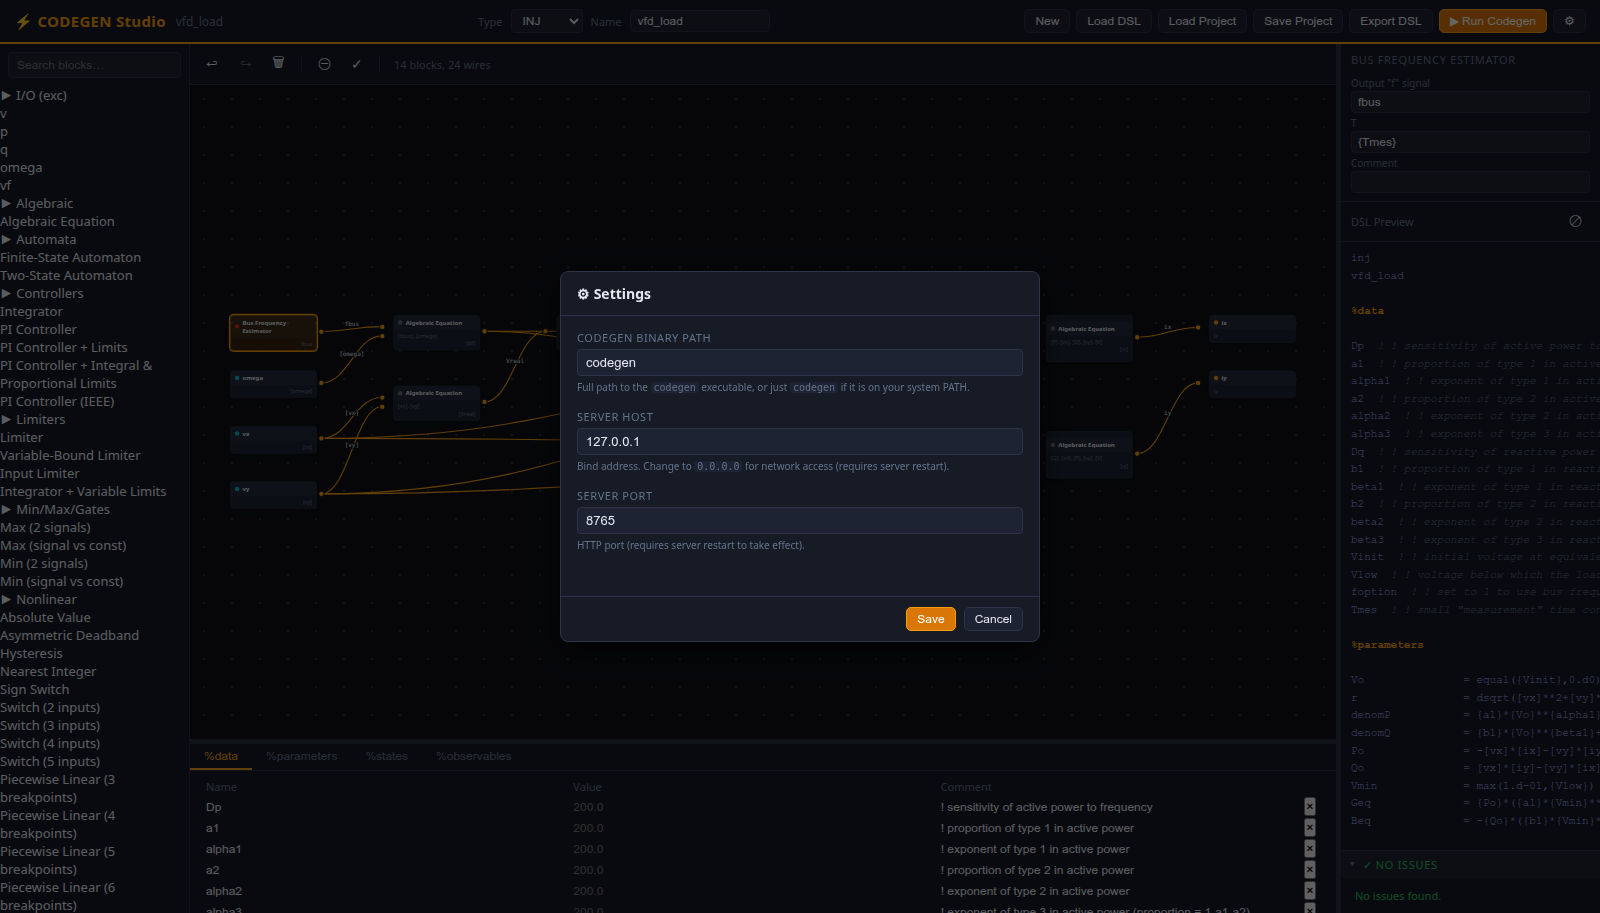
\includegraphics[width=0.98\linewidth]{figures/cg-studio-settings}
\caption{The Settings dialog over the editor, with three fields: codegen binary path set to codegen, server host set to 127.0.0.1, and server port set to 8765.}
\end{figure}

{\def\LTcaptype{none} % do not increment counter
\begin{small}\begin{longtable}[]{@{}
  >{\raggedright\arraybackslash}p{(\linewidth - 6\tabcolsep) * \real{0.3090}}
  >{\raggedright\arraybackslash}p{(\linewidth - 6\tabcolsep) * \real{0.2318}}
  >{\raggedright\arraybackslash}p{(\linewidth - 6\tabcolsep) * \real{0.4592}}
@{}}
\toprule\noalign{}
\begin{minipage}[b]{\linewidth}\raggedright
Setting
\end{minipage} & \begin{minipage}[b]{\linewidth}\raggedright
Default
\end{minipage} & \begin{minipage}[b]{\linewidth}\raggedright
Description
\end{minipage} \\
\midrule\noalign{}
\endhead
\bottomrule\noalign{}
\endlastfoot
\textbf{Codegen binary path} & \texttt{codegen} & Full path to the \texttt{codegen} executable \\
\textbf{Server host} & \texttt{127.0.0.1} & Bind address (change to \texttt{0.0.0.0} for network access) \\
\textbf{Server port} & \texttt{8765} & HTTP port \\
\end{longtable}\end{small}
}

Changes to host and port require a server restart. The codegen path takes effect immediately.

Settings are stored in a platform-specific config file:

\begin{itemize}
\tightlist
\item
  \textbf{Windows:} \texttt{\%LOCALAPPDATA\%\textbackslash{}cg-studio\textbackslash{}config.json}
\item
  \textbf{Linux/macOS:} \texttt{\textasciitilde{}/.config/cg-studio/config.json}
\end{itemize}

They can also be edited via the REST API at \texttt{/docs} (Swagger UI).

\begin{center}\rule{0.5\linewidth}{0.5pt}\end{center}

\section{Workflow Example: Building an AVR Model}\label{cg-studio:workflow-example-building-an-avr-model}

This walkthrough creates a simplified Automatic Voltage Regulator (AVR) as an EXC model.

\subsection{Step 1: Set up the model}\label{cg-studio:step-1-set-up-the-model}

\begin{enumerate}
\def\labelenumi{\arabic{enumi}.}
\tightlist
\item
  Select \textbf{EXC} from the Type dropdown
\item
  Type \texttt{simple\_avr} in the Name field
\end{enumerate}

\subsection{Step 2: Add data constants}\label{cg-studio:step-2-add-data-constants}

Switch to the \textbf{\%data} tab and add rows:

{\def\LTcaptype{none} % do not increment counter
\begin{small}\begin{longtable}[]{@{}lll@{}}
\toprule\noalign{}
Name & Value & Comment \\
\midrule\noalign{}
\endhead
\bottomrule\noalign{}
\endlastfoot
\texttt{KA} & & AVR gain \\
\texttt{TA} & & AVR time constant \\
\texttt{VREF} & & Reference voltage \\
\end{longtable}\end{small}
}

\subsection{Step 3: Place blocks}\label{cg-studio:step-3-place-blocks}

Drag the following blocks from the palette onto the canvas:

\begin{enumerate}
\def\labelenumi{\arabic{enumi}.}
\tightlist
\item
  \texttt{algeq}, to compute the voltage error
\item
  \texttt{tf1p}. a first-order transfer function for the AVR
\end{enumerate}

\subsection{Step 4: Connect and configure}\label{cg-studio:step-4-connect-and-configure}

\begin{enumerate}
\def\labelenumi{\arabic{enumi}.}
\tightlist
\item
  Connect the \texttt{algeq} output to the \texttt{tf1p} input
\item
  Select the \texttt{algeq} block and set its \textbf{Expression} to \texttt{\{VREF\}-{[}v{]}-avr1}
\item
  Select the \texttt{tf1p} block and:

  \begin{itemize}
  \tightlist
  \item
    Rename its output signal to \texttt{vf} (this is the mandatory EXC output)
  \item
    Set \textbf{K} to \texttt{\{KA\}} and \textbf{T} to \texttt{\{TA\}}
  \end{itemize}
\end{enumerate}

\subsection{Step 5: Define states}\label{cg-studio:step-5-define-states}

Switch to the \textbf{\%states} tab and add:

{\def\LTcaptype{none} % do not increment counter
\begin{small}\begin{longtable}[]{@{}lll@{}}
\toprule\noalign{}
Name & Init & Comment \\
\midrule\noalign{}
\endhead
\bottomrule\noalign{}
\endlastfoot
\texttt{avr1} & \texttt{vf/\{KA\}} & AVR integrator state \\
\end{longtable}\end{small}
}

\subsection{Step 6: Add observables}\label{cg-studio:step-6-add-observables}

Switch to the \textbf{\%observables} tab and add \texttt{vf}.

\subsection{Step 7: Export}\label{cg-studio:step-7-export}

\begin{enumerate}
\def\labelenumi{\arabic{enumi}.}
\tightlist
\item
  Click \textbf{``Export DSL''}, validation passes because \texttt{vf} is produced by the \texttt{tf1p} block
\item
  The downloaded \texttt{simple\_avr.txt} is ready for \texttt{codegen\ -tsimple\_avr.txt}
\item
  Or click \textbf{``Run Codegen''} to generate \texttt{exc\_simple\_avr.f90} directly
\end{enumerate}

\begin{center}\rule{0.5\linewidth}{0.5pt}\end{center}

\section{See Also}\label{cg-studio:see-also}

\begin{itemize}
\tightlist
\item
  \hyperref[ch-user_models]{User-Defined Models}, DSL file format and model framework
\item
  \hyperref[ch-libray_blocks]{CODEGEN Blocks}, complete block reference
\item
  \hyperref[doc:codegen-examples]{CODEGEN Model Examples}, annotated model files for all four types
\end{itemize}
